\section{Path Following Algorithm}\label{sec:pathfollower}
The path generated is approximated by straight line segments connected by the calculated waypoints. The vessel then follows these in order to track the path and cover the area in which the measurements are to be taken. This approximation is suitable as the bathymetric measurements are usually taken in straight line paths. Straight line segments on the curved paths are not required as the curved paths are outside of the area of interest. If curved paths were required, the solution would be to sample the path with higher frequency in curved sections. \autoref{fig:pathandwaypoints} shows an example of how a path is approximated by straight line segments and waypoints.
\begin{figure}[H]
	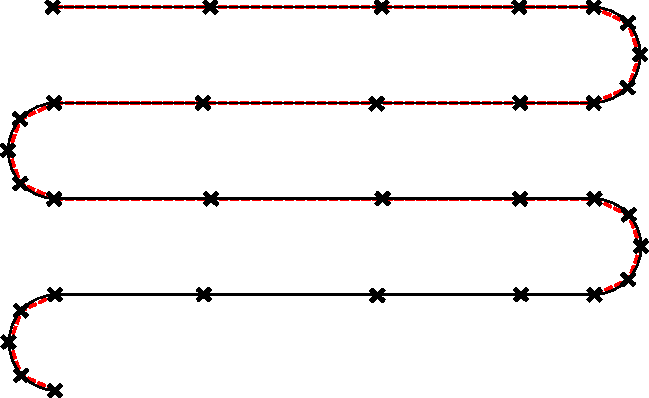
\includegraphics[width=0.6\textwidth]{figures/pathandwpts}
	\caption{A predefined path and its approximation as straight line segments using waypoints.}
	\label{fig:pathandwaypoints}
\end{figure}
The algorithm starts by considering the first two waypoints in the path. The yaw reference given to the state space controller is calculated based on the crossing point between the straight line segment that joints the waypoints and a circle centered in the position of the boat. \autoref{fig:LOSalgorithm} shows how this crossing point is obtained. The crossing point is also called LOS (Line Of Sight) point and is found using the equations of the circle and of the straight line as
%
\begin{flalign}
	(&x_\mathrm{los}-x_\mathrm{n})^2 + (y_\mathrm{los}-y_\mathrm{n})^2 = R^2, \label{eq:circle} \ \\
	&y_\mathrm{los}-y_\mathrm{k} = \frac{y_\mathrm{k+1}-y_\mathrm{k}}{x_\mathrm{k+1}-x_\mathrm{k}}(x_\mathrm{los}-x_\mathrm{k}) \label{eq:line} 
\end{flalign}
\begin{where}
	\va{R}{is the radius of the circle centered at the vessel position}{}
	\va{[x_\mathrm{los},y_\mathrm{los}]}{is the crossing point between the circle around the vessel and the straight line that joins the waypoints}{}
	\va{[x_\mathrm{k},y_\mathrm{k}]}{is the first waypoint in the currently followed path segment}{}
	\va{[x_\mathrm{k+1},y_\mathrm{k+1}]}{is the second waypoint in the currently followed path segment}{}
	\va{[x_\mathrm{n},y_\mathrm{n}]}{is the position of the vessel in the NED frame}{}
\end{where}
%
\begin{figure}[H]
	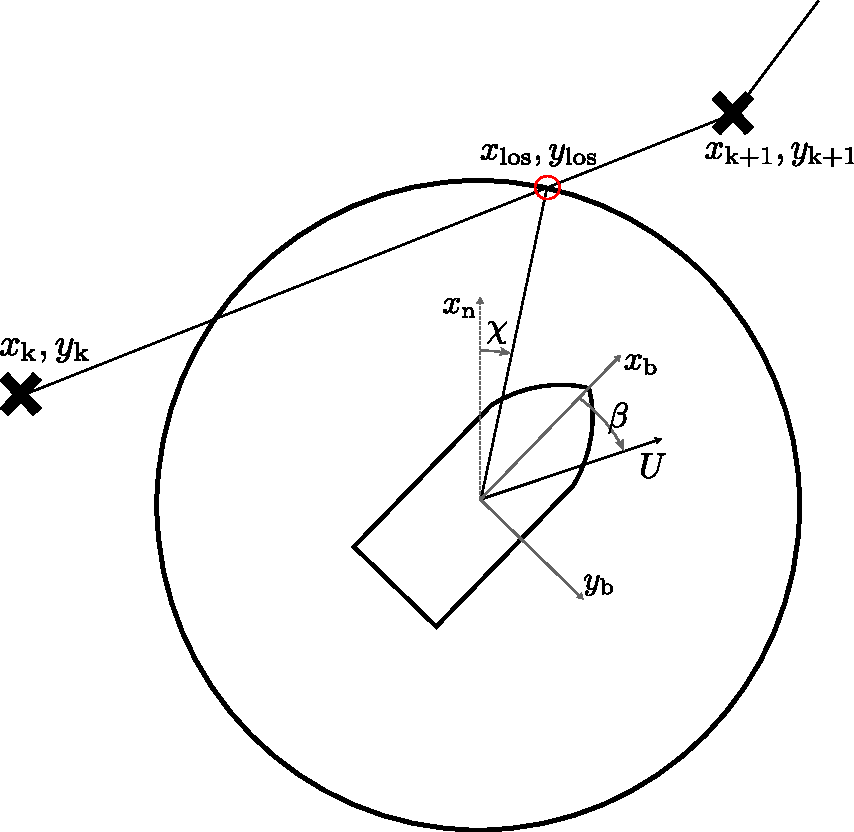
\includegraphics[width=0.5\textwidth]{figures/LOSalgorithm}
	\caption{Algorithm used to find the yaw reference for the state space controller in order to follow a path.}
	\label{fig:LOSalgorithm}
\end{figure}
The LOS point is then used to calculate $\chi$ as the angle from the $x_\mathrm{n}$ axis and the line joining the position of the vessel and the LOS point. See \eqref{eq:chi}. This can be directly used as the reference for yaw, $\psi_\mathrm{ref}$, in the state space controller. This disregards the possibility of disturbances and assumes that the velocity vector of the vessel is aligned with the $x_\mathrm{b}$ axis. This is in general not true as disturbances like wind or waves would generate some speed also in the $y_\mathrm{b}$ axis direction. The reference for yaw is then adjusted by subtracting the angle that the velocity vector has with respect to the $x_\mathrm{b}$ axis as seen in \eqref{eq:beta} and \eqref{eq:psiref}. 

This approach tries to make the vessel velocity vector point towards the LOS point.
%
\begin{flalign}
	\chi &= \arctan\left(\frac{y_\mathrm{los}-y_\mathrm{n}}{x_\mathrm{los}-x_\mathrm{n}}\right), \label{eq:chi} \ \\
	\beta &= \arctan\left(\frac{\dot{y}_\mathrm{b}}{\dot{x}_\mathrm{b}}\right) \label{eq:beta}, \ \\
	\psi&_\mathrm{ref} = \chi - \beta. \label{eq:psiref}
\end{flalign}
\begin{where}
	\va{\chi}{is the angle between the $x_\mathrm{n}$ axis and the LOS point}{}
	\va{\beta}{is the angle between the velocity vector of the vessel and the $x_\mathrm{b}$ axis}{}
\end{where}
%
The algorithm relies on the path and the circle defined around the boat to cross at the LOS point. 

If the vessel is positioned far from the path such that the circle does not intersect it, then the algorithm uses the next waypoint as LOS point. Once the vessel gets closer to the path, the LOS point is calculated as described above.

The yaw reference, $\psi_\mathrm{ref}$, given to the controller in \ref{innercontrol} ensures that the vessel will follow the desired LOS.

In order to follow all the path, a way to change which two waypoints define the current path segment needs to be established. Several possibilities can be considered but all of them change active waypoints when the vessel gets close enough to the waypoint that defines the end of the segment. In the project at hand, the distance to the waypoint is evaluated as the distance from the waypoint to the intersection point of the path segment and a perpendicular line to the segment that passes through the vessel position. This distance is depicted in \autoref{fig:changewaypoints}.
\begin{figure}[H]
	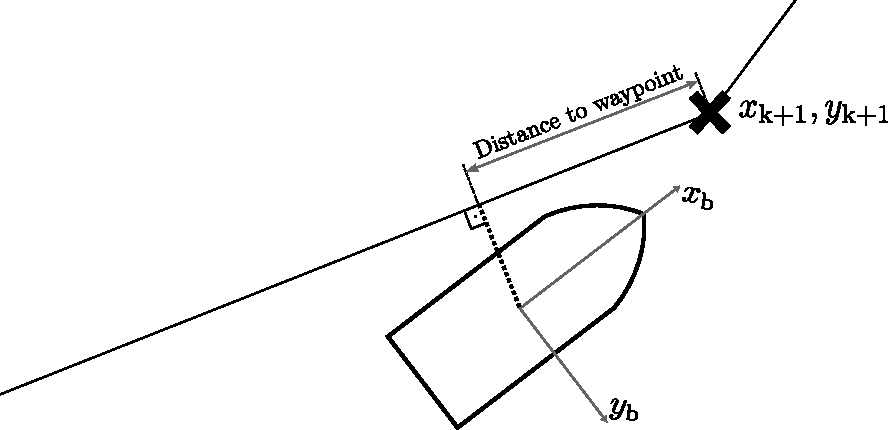
\includegraphics[width=0.6\textwidth]{figures/LOSalgorithmdistancewp}
	\caption{The distance considered when defining the criterion to change to new waypoints.}
	\label{fig:changewaypoints}
\end{figure}
With this approach, the vessel will always try to move forward in the path although a waypoint position has not been precisely attained. % This avoids situations like the one shown in \autoref{fig:goingbackapproach} where the vessel turns around in order to hit the waypoint precisely.
This could be caused by a sudden disturbance experienced by the vessel and, in general, it is desired to keep following the path rather than turning around to hit the waypoint. In most cases, the vessel itself is going to be close to the waypoint when the change occurs. This can be seen in the simulation plots presented below. 

\subsection{Path Following Algorithm Simulation}

\fxnote{Do not include many graphs now because we will probably redo them. Just some dummy ones.} 
\fxnote{Maybe we could include the result also with different low level controllers}
The path following algorithm has been tested in the same path and considering different settings for the algorithm. In all cases, the radius of the circle defined around the vessel is 5 m and the distance in which the active waypoints are changed is 3 m. 

In \autoref{fig:simpleLOSalgorithm} and \ref{fig:simpleLOSalgorithmdisturbance} the results of the algorithm are presented when considering the simpler case in which $\psi_\mathrm{ref} = \chi$, that is, assuming the velocity of the vessel is pointing along the $x_\mathrm{b}$ direction. In the first graph the path is followed precisely as the assumption regarding the velocity vector holds,  whereas in the second, the constant disturbance imposes an offset in the position of the vessel.
\begin{figure}[H]
	\captionbox  %<--use captionbox instead if no global caption is needed
	{               %                                \%-%-%-%-%-%-%\
	 	Performance of the path following algorithm based on $\psi_\mathrm{ref}=\chi$.                %\
		\label{fig:simpleLOSalgorithm}                                  %\
	}                                                                 %\
	{                                                                  %\
		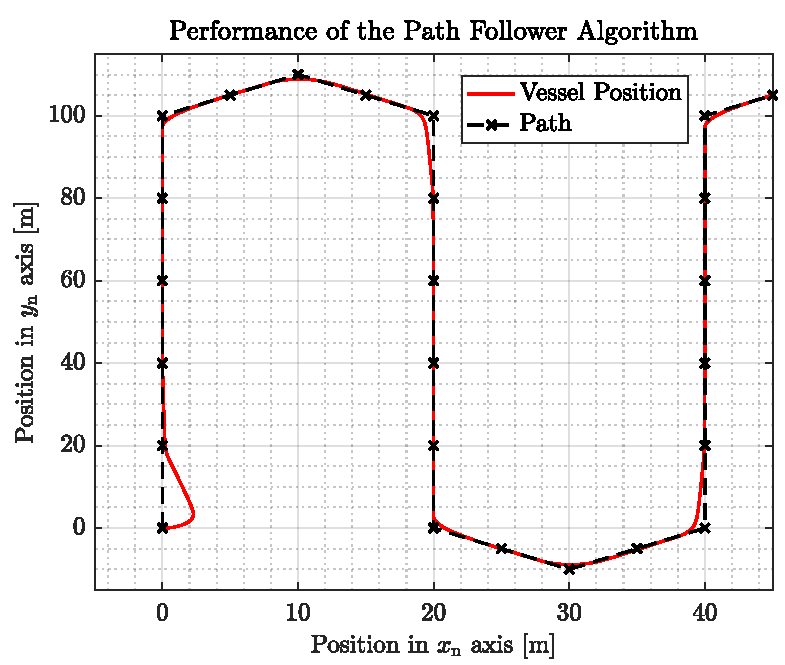
\includegraphics[width=.45\textwidth]{figures/pathfollowingsimple}         %\
	}                                                                    %\
	\hspace{5pt}                                                          %\
	\captionbox  %<-----------------------------------------------------%\
	{       
		Performance of the path following algorithm based on $\psi_\mathrm{ref}=\chi$. The vessel is experiencing a constant disturbance force of 1 N applied with an angle of $\pi/2$.                                                                  %\                         %\
		\label{fig:simpleLOSalgorithmdisturbance}                                     %\
	}                                                                           %\
	{                                                                            %\
		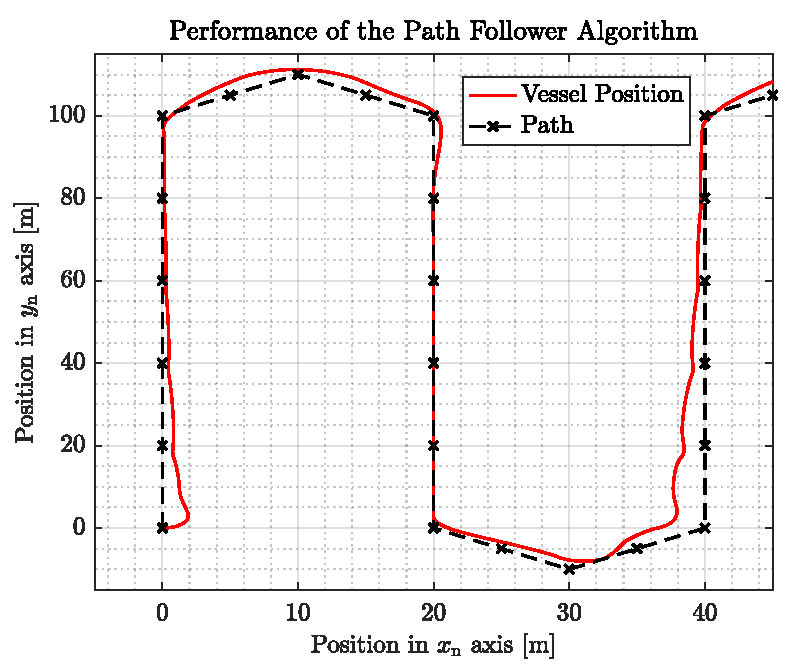
\includegraphics[width=.45\textwidth]{figures/pathfollowingsimpledist}            %|
	}                                                                             %|
\end{figure}
When the information of the vessel velocity is used to calculate the reference angle, $\psi_\mathrm{ref}$, the disturbance is rejected. This is seen in \autoref{fig:normalLOSalgorithmdisturbance}, where the vessel is experiencing the same disturbance as in \autoref{fig:simpleLOSalgorithmdisturbance}. In this case, the offset in position has been corrected and the path is precisely followed.
\begin{figure}[H]
	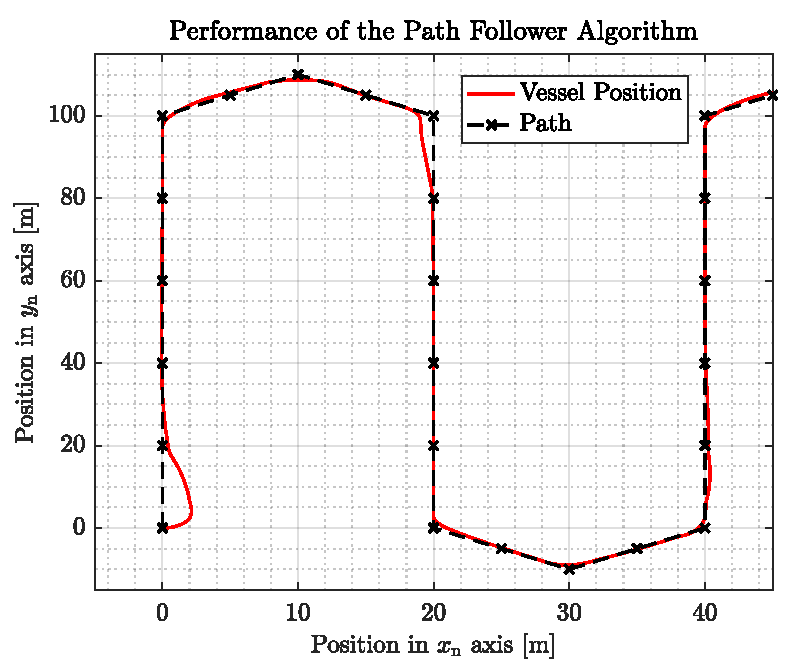
\includegraphics[width=0.5\textwidth]{figures/pathfollowingcomplex}
	\caption{Performance of the path following algorithm based on $\psi_\mathrm{ref}=\chi-\beta$. The vessel is experiencing a constant disturbance force of 1 N applied with an angle of $\pi/2$.}
	\label{fig:normalLOSalgorithmdisturbance}
\end{figure}
According to the results of the simulations, it can be said that the vessel hits the waypoints precisely when they are part of a straight line section of the path. In curved sections, the vessel joins smoothly the straight line segments that approximate the curve. In many cases, and especially for bathymetric measurements the algorithm can be considered suitable.

	



